Most reconstruction methods rely on an accurate tracking of the ultrasound probe, and there are several ways to obtain this. Most methods use either electromagnetic, optical, mechanical or acoustic sensors, but an alternative is to estimate the orientation from the ultrasound scans themselves. Such sensorless tracking can be done by analyzing speckle noise in the scans using decorrelation or linear regression techniques. However, sensorless systems do not offer the same accuracy as with actual sensors \cite{mercier2005}.

Mechanical tracking methods involve attaching the probe to structures with certain degrees of freedom, or letting a machine move the probe automatically. Disadvantages with this method is the reduced freedom and that additionally only one probe at the time can be tracked. Acoustic tracking uses sound emitters and receivers. The position can be tracked by measuring the time it takes for the sound to reach the receiver, or by measuring the relative phase shift when moving the probe. Disadvantages include the required line of sight for the sound waves, and varying speed of sound depending on factors such as temperature and pressure. Electromagnetic tracking systems measure current induced by moving a receiver in an electromagnetic field. This method has the advantage of being resistant against occlusion, but metallic objects as well as power sources or CRT monitors can distort the field.

An optical tracking system such as the one used for data collection for our thesis is shown in Figure \ref{fig:tracking_system}. Spheres that reflect infrared light are attached to the probe, and two cameras record the reflected infrared light. The position of the spheres relative to the cameras can then be used to estimate the location and orientation of the probe. Obviously, the system requires that the probe is in line of sight from the cameras.

	\begin{figure}[h]
	\centering
	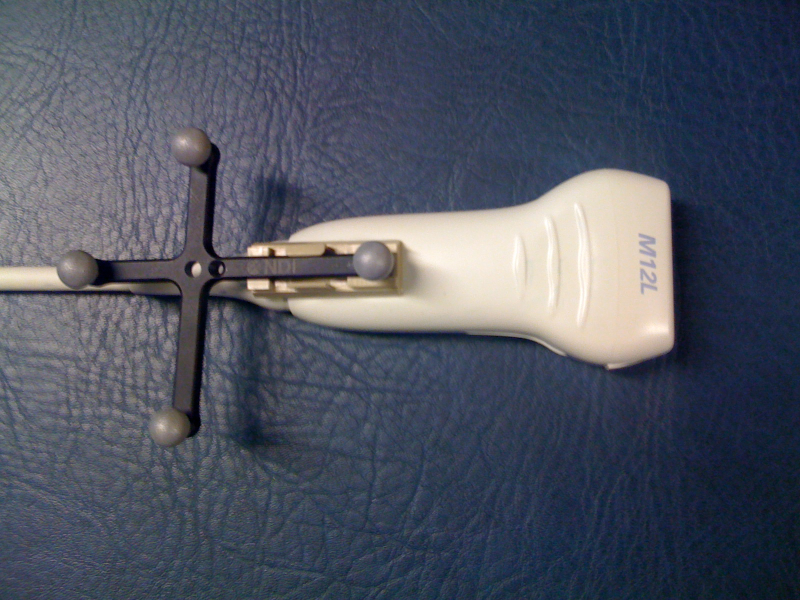
\includegraphics[height=0.23\textheight]{graphics/tracking_system_1.png}
	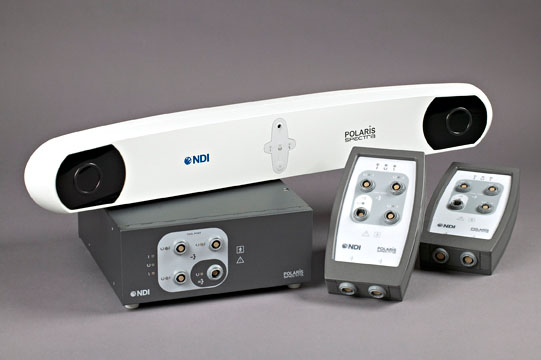
\includegraphics[height=0.23\textheight]{graphics/tracking_system_2.png}
	\caption[Linear array probe and optical tracking system]{GE M12L linear array probe (GE Healthcare, Waukesha, Wisconsin, USA) with tracking frame and Polaris Spectra optical tracking system (Northern Digital, Waterloo, Canada) (Photo of Polaris Spectra used with permission from Northern Digital Inc.)}
	\label{fig:tracking_system}
	\end{figure}